\newcommand\codefamily\sffamily
\lstset{language={[Sharp]C},mathescape=true,flexiblecolumns=true,morekeywords={Requires,Ensures,Invariant},basicstyle=\codefamily\small,literate={->}{{$\rightarrow$}}{2}{<<}{{$\langle$}}{2}{>>}{{$\rangle$}}{2}{!}{{\textbf{!}}}{2},frame=lines,moredelim=[is][\itshape]{@}{@},captionpos=b,numberstyle=\tiny,stepnumber=1,numbersep=2pt}

\section{Adding the Contract Library Reference}
If you are using Visual Studio 2008, or if you for 
some reason want to target a pre-v4 .NET runtime, then you need to:
\begin{itemize}
\item Change the target framework of the project.
\item Manually add a reference to Microsoft.Contracts.dll
\end{itemize}
Otherwise, you may skip this section and go directly the next section!

To add the reference, open the
\textsf{\SolutionName{}} solution and right-click on
\textsf{References} in the \textsf{\ProjectName{}} project and
select \textsf{Add Reference}. Find the \textsf{Microsoft.Contracts}
library in the \textsf{.NET} tab as shown below and click OK.
\begin{center}
  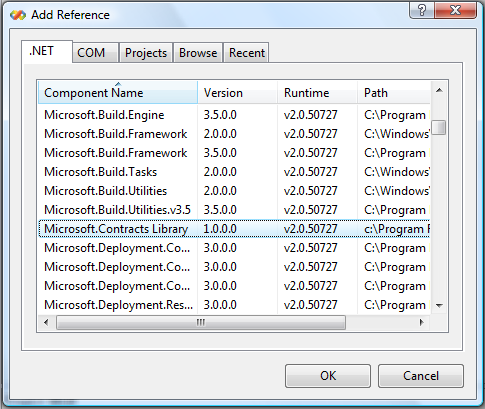
\includegraphics[width=.7\columnwidth]{../Common/addRef.png}
\end{center}

